% !TEX encoding = UTF-8 Unicode
\chapter{Additional results and sensitivity analysis}     % numérotée
\label{chap-Annex}                   % étiquette pour renvois (à compléter!)

\section{Algorithms} \label{section:annex-alg-KF}

\begin{itemize}
	\item Kalman filter update algorithm
	\item Multi-model algorithms.
\end{itemize}

\section{Tuning of KF3 for MIMO linear system} \label{section:annex-sim-2-KF-tuning}

As described in Chapter \ref{chap-simulation}, a standard Kalman filter was tuned to minimize the RMSE of the output estimates using 5000 data samples from the $2\times2$ linear system. Since the system is symmetrical and the two RODDs have the same parameters, it was assumed that the two observer parameters, $\sigma_{w_p,1,\text{opt}}$ and $\sigma_{w_p,2,\text{opt}}$ must also be identical. This assumption simplified the search process since only one optimum value needed to be found.

Figure \ref{fig:sim-sys-2x2-KF3-tuning-sens} shows the variation in the RMSEs of the four model state estimates with the parameters. In this case, the choice of optimal parameter value was not as straight-forward as in the case of the SISO system with one RODD. The minimum RMSE for each state occurs at different values of  1 and 2 is achieved when $\sigma_{w_p,1,\text{opt}}=\sigma_{w_p,2,\text{opt}}=0.0075$

\begin{figure}[htp]
	\centering
	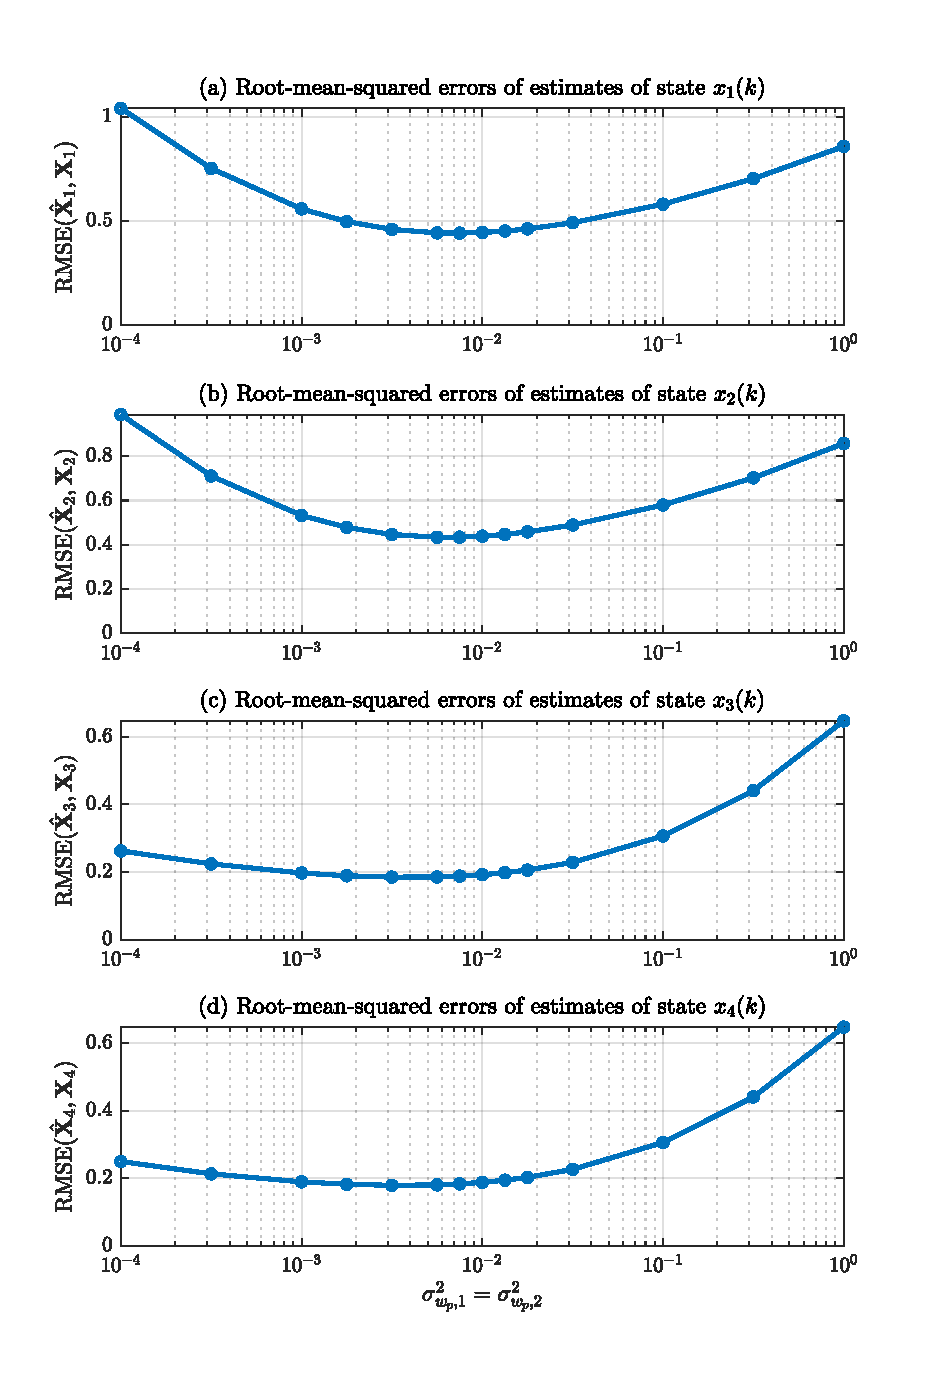
\includegraphics[width=14cm]{images/rod_obs_sim2_3KF_Q_seed_0.pdf}
	\caption{Tuning of Kalman filter KF3 – $2\times2$ system}
	\label{fig:sim-sys-2x2-KF3-tuning}
\end{figure}
	

\section{Sensitivity analyses}

\subsection{Pseudo-random numbers}

Many of the simulation results are sensitive to the initialization of the pseudo-random number generator (PRNG) used to simulate random processes. In particular, the RODD step disturbance (\ref{eq:wpk2}) is simulated by generating three pseudo-random sequences, two random noise sequences and a random binary sequence to simulate the infrequent shocks.  Since the random shocks are infrequent and tend to have a large magnitude, their effect on the simulation results can be significant.

To visualize this effect, consider the plot in Figure \ref{fig:rod-obs-sim-1-3KF-seed-crmse-statsplot}. This shows the RMSE of the output estimates of the three Kalman filters described in Section \ref{sim-obs-lin-1} for 10 simulations, each generated with a different \textit{seed}—the seed is a scalar argument used to initialize the PRNG algorithm in a unique state. The RMSE is calculated for every simulation duration, $t_N=0.5,1,1.5,...,2500$. The coloured areas represent the range between the lowest and the highest RMSE obtained for the 10 different simulations of each duration. The dark lines represent the median values.

\begin{figure}[htp]
	\centering
	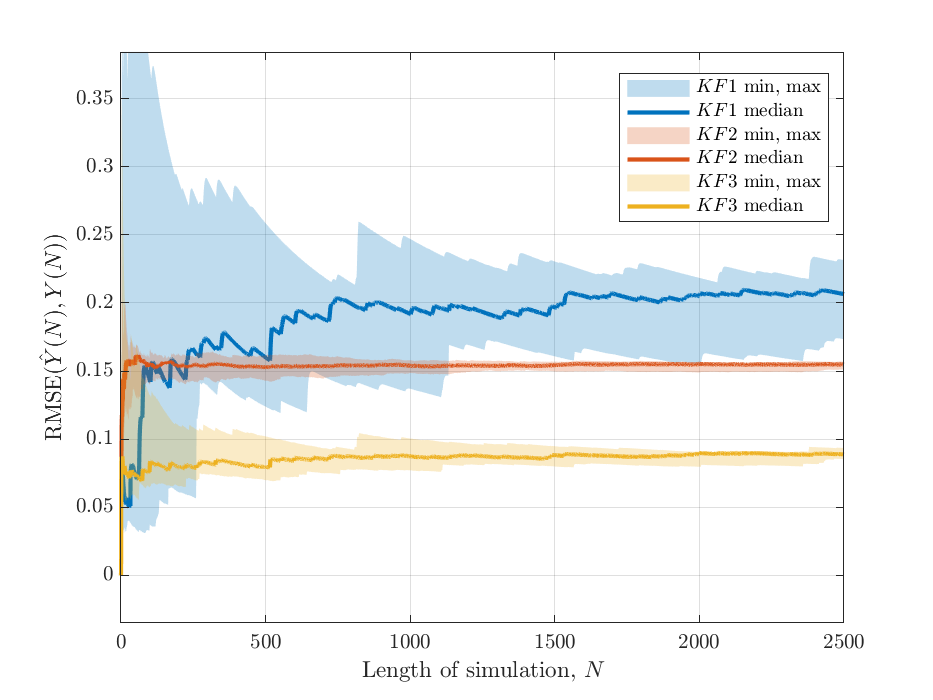
\includegraphics[width=14cm]{images/rod_obs_sim1_3KF_seed_crmse_statsplot.pdf}
	\caption{Effect of random variables on the RMSE results.}
	\label{fig:rod-obs-sim-1-3KF-seed-crmse-statsplot}
\end{figure}

As expected, the differences in the results due to PRNG initialization are smaller the greater the length of the simulation. However, the magnitude of the differences is not the same for each observer. The RMSE values of KF1, which has the lowest gain, are more sensitive to the random initialization than the other two filters. Therefore it is not possible to estimate the expected value of the RMSE of KF1 from a single simulation of this duration---a longer simulation or a larger number of simulations would be needed. On the other hand, the variations in the RMSEs of KF2 and KF3 are significantly lower. After the full length of the simulations ($t_N=2500$), the RMSE of KF2 is between -0.0039 (-2.5\%) and 0.0019 (1.3\%) of the median value, which is $0.1550$.  That of KF3 is between -0.0035 (-4.0\%) / 0.0047 (5.3\%) of the median, 0.0889.  Therefore it is reasonable to conclude that the RMSE of KF3 is consistently about 0.05 lower than that of KF2. Note that the RMSEs of KF2 and KF3 reported in Section \ref{sim-obs-lin-1} are \textcolor{red}{0.XXXX and 0.XXXX}. These values are both within the minimum and maximum values from this sensitivity analysis (in fact, the simulation output used to produce the main results is one of the 10 shown here).

A similar sensitivity analysis was carried out on the results of the Kalman Filter tuning shown in Figure \ref{eq:sim-sys-siso-KF3-Q}, where KF3 was tuned using a set of 5000 input-output samples from the system. Figure \ref{fig:sim-sys-siso-KF3-sensitivity} shows the variation in this result when ten different sets of pseudo-random simulation data are used.  Although there is considerable variation in the RMSE values for each parameter value, the best overall choice of $\sigma_{w_p}$ to achieve the lowest average error across all 10 simulations was found to be the same as that of the single simulation (0.01).

\begin{figure}[htp]
	\centering
	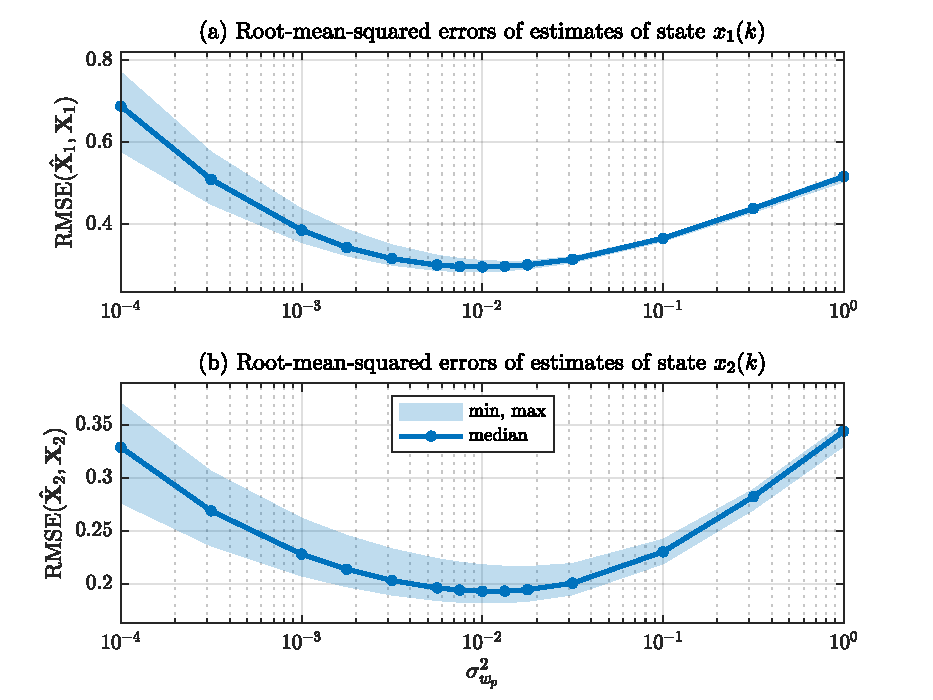
\includegraphics[width=14cm]{images/rod_obs_sim1_3KF_Q_statplot.pdf}
	\caption{Sensitivity of Kalman filter tuning – SISO system}
	\label{fig:sim-sys-siso-KF3-sensitivity}
\end{figure}

Figure \ref{fig:sim-sys-2x2-KF3-tuning-sens} shows the results of a similar sensitivity analysis on the results presented in Figure \ref{fig:sim-sys-2x2-KF3-tuning}.

\begin{figure}[htp]
	\centering
	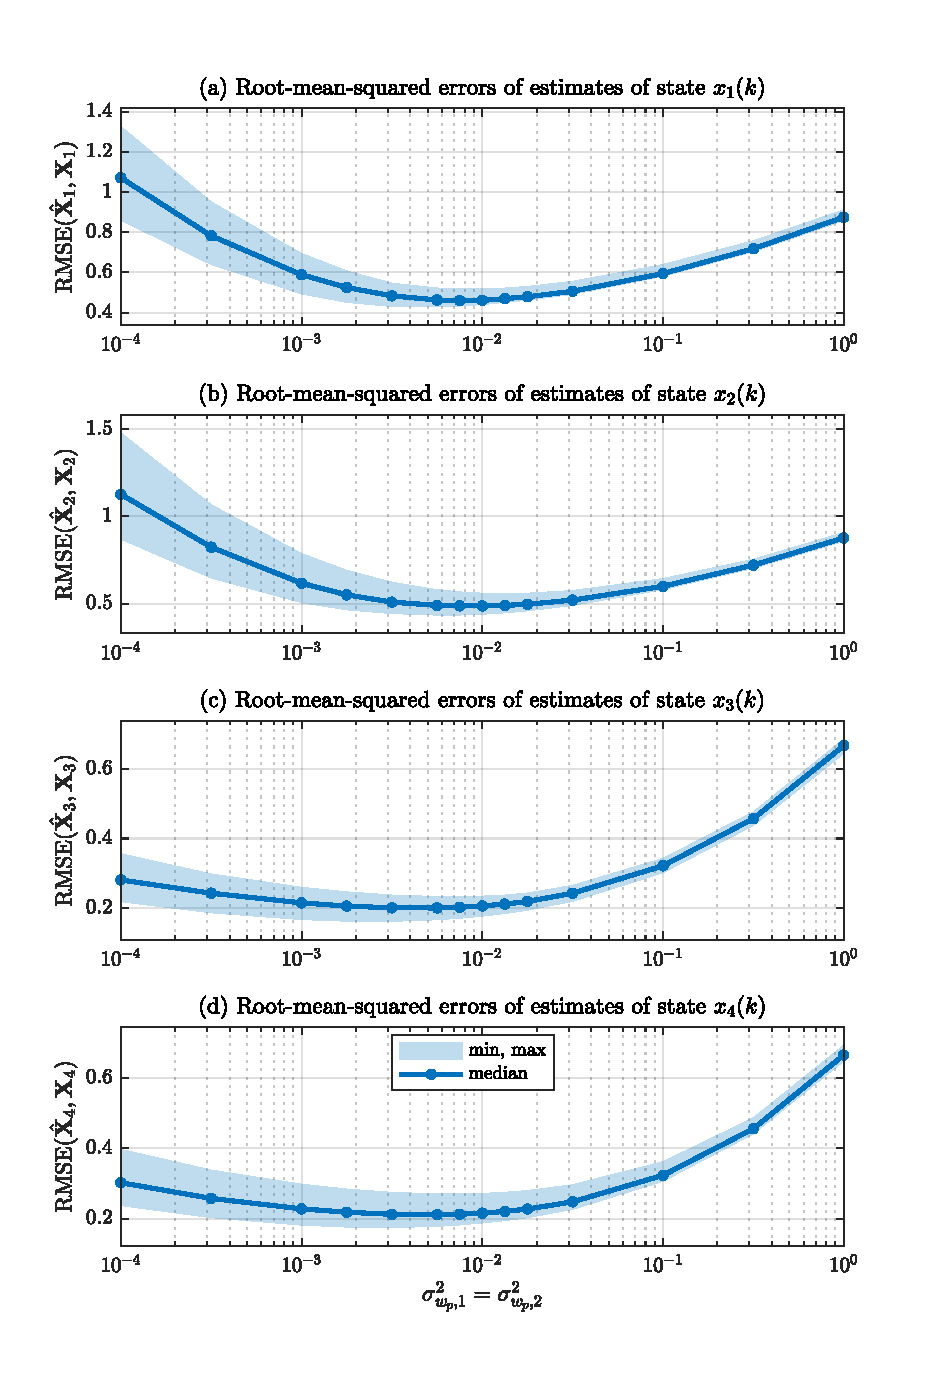
\includegraphics[width=14cm]{images/rod_obs_sim2_3KF_Q_statplot.pdf}
	\caption{Sensitivity of Kalman filter tuning – $2\times2$ system}
	\label{fig:sim-sys-2x2-KF3-tuning-sens}
\end{figure}

